\documentclass{beamer}
\DeclareGraphicsExtensions{.pdf,.jpg,.eps}
\definecolor{grisbleu}{rgb}{0.85,0.85,1}
\mode<beamer>{%
  \beamertemplatesolidbackgroundcolor{grisbleu}
 % \usetheme{Paloalto}
  %\usetheme{Montpellier}
  \usetheme{Pittsburgh}
  \usefonttheme{serif,professionalfonts}
}

\mode<trans>{\usetheme{Pittsburgh}}
%%%%%%%%%%%%%%%%%%%%%%%%%%%%%%%%%%%%%%%%%%%%%%%%%%%%%%%%%%%%%%%%%

%\DeclareGraphicsRule{*}{mps}{*}{} % Figures MetaPost

\usepackage{pgf,pgfarrows,pgfnodes}

%\usepackage{pdfcolmk}

% Options pour hyperref.sty
\hypersetup{pdfnewwindow=false}
%\hypersetup{pdfpagemode=FullScreen}
 \setbeamercovered{dynamic}
   \setbeamertemplate{background canvas}[vertical shading][bottom=red!10,top=blue!10]
\usepackage{amsmath}

\usepackage{xmpmulti}
%\usepackage[latin1]{inputenc}
\usepackage[T1]{fontenc}
%\usepackage[oldstyle,upright]{fourier}
\usepackage[upright]{fourier}% Si on n'a pas les compl\'{e}ments expert...
% sf = helvetica scaled 88%
\usepackage[scaled=.88]{helvet}
% tt = lmtt
\newcommand\X{\mathcal{X}}
\newcommand\Z{\mathcal{Z}}
\newcommand\M{\mathcal{M}}
\newcommand\Lv{\mathcal{L}}
\newcommand\E{\mathbb{E}}
\newcommand\la{\ln{\bf \alpha}}
\newcommand{\Xcal}{\mathcal{X}}
\newcommand{\Zbf}{{\bf Z}}
\newcommand{\Vbf}{{\bf V}}
\newcommand{\Xbf}{{\bf X}}
\newcommand{\Zcal}{\mathcal{Z}}
\newcommand{\wbf}{{\bf w}}
\newcommand{\alphabf}{\text{\mathversion{bold}{$\alpha$}}}
\newcommand{\pibf}{\mbox{\mathversion{bold}{$\pi$}}}
\newcommand{\Pibf}{\mbox{\mathversion{bold}{$\Pi$}}}
\newcommand{\thetabf}{\mbox{\mathversion{bold}{$\theta$}}}
\newcommand{\Thetabf}{\mbox{\mathversion{bold}{$\Theta$}}}
\newcommand{\taubf}{\mbox{\mathversion{bold}{$\tau$}}}
\newcommand{\pibar}{\bar{\pi}}
\newcommand{\Qcal}{\mathcal{Q}}
\newcommand{\RX}{\mathcal{R}_{\Xbf}}
\newcommand{\Lcal}{\mathcal{L}}
\renewcommand{\ttdefault}{lmtt}
\newcommand{\Abf}{{\bf A}}
\newcommand{\Bcal}{\mathcal{B}}
\newcommand{\C}{C}
\newcommand{\Esp}{\mathbb{E}}
\newcommand{\eps}{\varepsilon}
\newcommand{\epsbar}{\overline{\eps}}
\newcommand{\etabar}{\overline{\eta}}
\newcommand{\fbf}{{\bf f}}
\newcommand{\Gcal}{\mathcal{G}}
\newcommand{\Hbf}{{\bf H}}
\newcommand{\Ibb}{\mathbb{I}}
\newcommand{\Kcal}{\mathcal{K}}
\newcommand{\lambdabar}{\overline{\lambda}}

\newcommand{\Mcal}{\mathcal{M}}
\newcommand{\Ncal}{\mathcal{N}}
\newcommand{\Pcal}{\mathcal{P}}

\setbeamercolor{monalerte}{fg=blue}

\newcommand{\rhobar}{\overline{\rho}}
\newcommand{\Sbf}{{\bf S}}
\newcommand{\Vcal}{\mathcal{V}}
\newcommand{\Vsf}{\mathsf{V}}

%\newcommand{\Zbf}{{\bf Z}}
%%%% tableau display�e � chaque case %%%%
\newenvironment{disarray}%
 {\everymath{\displaystyle\everymath{}}\array}%
 {\endarray}

%\usepackage[frenchb]{babel}
\mode<beamer>
\makeatletter
\DeclareRobustCommand\sfrac[1]{\@ifnextchar/{\@sfrac{#1}}%
                                          {\@sfrac{#1}/}}
\def\@sfrac#1/#2{\leavevmode\kern.1em\raise.5ex
         \hbox{$\m@th\mbox{\fontsize\sf@size\z@
                           \selectfont#1}$}\kern-.1em
         /\kern-.15em\lower.25ex
          \hbox{$\m@th\mbox{\fontsize\sf@size\z@
                            \selectfont#2}$}}
\makeatother

\newcommand{\Indic}{{\mathbb I}}
% Texte
\usepackage{lscape,fancyhdr, rotating, enumerate,psfig}
%
\title{Mixture models for random graphs}
\author[J.J. Daudin]{Jean-Jacques Daudin \\
 UMR AgroParisTech-INRA518}

\date{ GDR Statistique et Sante, \\ 13 November 2008,}
\begin{document}
\begin{frame}
\titlepage
\begin{tabular}{lr}
 \includegraphics[height=1.5cm ] {SSB.png} & \includegraphics[height=1.5cm ] {logagroptech.png} \\
\end{tabular}
\end{frame}


\section{introduction}
\begin{frame}
\frametitle{Why do people represent data by a network (1) ?}
\begin{tabular}{p{5cm}p{5cm}}
  \vspace{0cm} \hspace{-1.5cm}
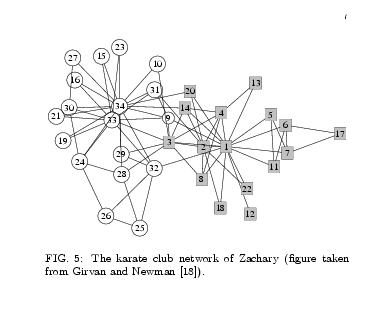
\includegraphics[scale=0.5]{graphe_karate.png}\\ &
\vspace{-6cm} \begin{itemize}
    \item Real networks do exist: electric, transport or www
    networks...They have been represented for a long time by
    virtual networks.
    \item Virtual network is a nice way for representing or even "modelling"  many
    scientific phenomenons: social relations, metabolic pathways,
    chemical reactions...
\end{itemize}     \\

\end{tabular}

\end{frame}

\begin{frame}
\frametitle{Why do people represent data by a network (2) ?}
\begin{tabular}{p{7cm}p{3.5cm}}
  \vspace{-0.5cm}
\includegraphics[scale=0.32] {Barabasi6.png} & \begin{itemize}
    \item an overall representation of the interactions between many nodes
    \item the plot reveals the topology of the networks
    \item nodes may be colored, adding more information
\end{itemize}     \\

\end{tabular}

\end{frame}





\begin{frame}
\frametitle{An unusual data set structure}

\begin{tabular}{cc}

  % after \\: \hline or \cline{col1-col2} \cline{col3-col4} ...
  Usual i.i.d. structure & \alert{Structure for relational data} \\

  \begin{tabular}{|c|c|c|c|c|}
    \hline
    % after \\: \hline or \cline{col1-col2} \cline{col3-col4} ...
    item &$X_1$ & ... & ... & $X_p$\\
    \hline
    1 & $x_{11}$ & ... & ... & $x_{1p}$ \\
    2 & $x_{21}$ & ... & ... & $x_{2p}$ \\
    . & . & . & . & . \\
    $n$ & $x_{n1}$ & ... & ... & $x_{np}$ \\
    \hline
  \end{tabular}
     &
     \alert{
\begin{tabular}{|c|c|c|}
    \hline
    item1 & item2 & $R$ \\
    \hline
    1 & 2 & $r_{12}$  \\
    1 & 3 & $r_{13}$ \\
    . & . & .  \\
    $n-1$ & $n$ & $r_{n-1,n}$  \\
    \hline
  \end{tabular}
  }
  \\
\end{tabular}

\begin{itemize}
    \item In the relational data set, the core information is the relation
between two items.
    \item lines are not independent
    \item the data structure is similar to distance, similarity, covariance or
    correlation matrices
   % \item \alert{the two types of structures may be combined: information
   % about items + information about relations between them.}
\end{itemize}

\end{frame}





\begin{frame}
\frametitle{What do we want?}
A simple representation of a complex graph, using meta-vertices and meta-edges.
\begin{tabular}{p{5cm}p{5cm}}
\hspace{-2cm}
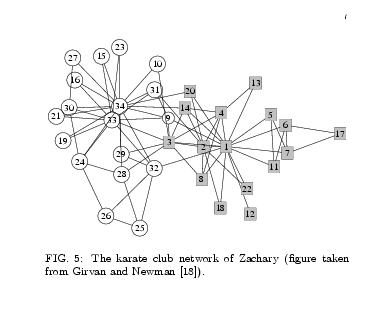
\includegraphics[scale=0.5]{graphe_karate.png}
    &
  \vspace{-5cm}
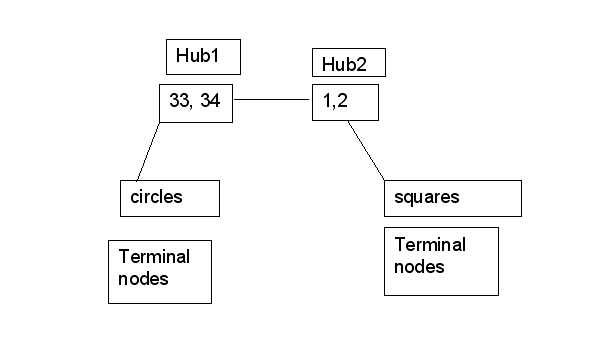
\includegraphics[scale=0.3]{karate-simple.png} \\
\end{tabular}

\end{frame}


\section{Nodes clustering}

\begin{frame}
\frametitle{Mixtnet: a mixture model for random graphs}
\begin{itemize}
\item
$i=1,n$ nodes
\item $q=1,Q$ classes
\item $X_{ij}=1$ if there is an edge from node $i$ to node $j$.
\item
      $Z=Z_{iq}$ discrete latent variable, $Z_{iq}=1$ if node $i$ pertains to class $q$
      \item $(Z_{i1},Z_{i2}...Z_{iQ}) \sim \M(1,\alpha_1,\alpha_2,...\alpha_Q)$
      \item Conditionally to $Z$, $X_{ij}$ are independent Bernoulli RV with
        $$P(X_{ij}=1/Z_i=q,Z_j=l)=\pi_{ql}$$
        \end{itemize}


\end{frame}

\begin{frame}
\frametitle{Mixnet: a flexible model}
  \begin{table}[h]
    \begin{center}

      \begin{tabular}{lccc}

        \hline
        Description & Graph & $Q$ & $\pibf$ \\


        \hline
        \begin{tabular}{p{2cm}} Erdos, no cluster \end{tabular}

        & \begin{tabular}{c}
          \includegraphics[height=1.2cm,width=2.3cm]{FigNetworks-Erdos.pdf}
        \end{tabular}

        & 1
        &  $p$ \\


        \hline
        \begin{tabular}{p{2cm}} Hubs \end{tabular}

        & \begin{tabular}{c}
          
\includegraphics[height=1.5cm,width=2.3cm]{FigNetworks-Star.pdf}
        \end{tabular}

        & 4

        & $\left( \begin{array}{cccc} 0&1&0&0\\ 1&0&1&0\\0&1&0&1\\0&0&1&0\\
          \end{array} \right)$
         \\


        \hline \begin{tabular}{p{2cm}}  cluster in "usual sense"  \end{tabular}

        & \begin{tabular}{c}
          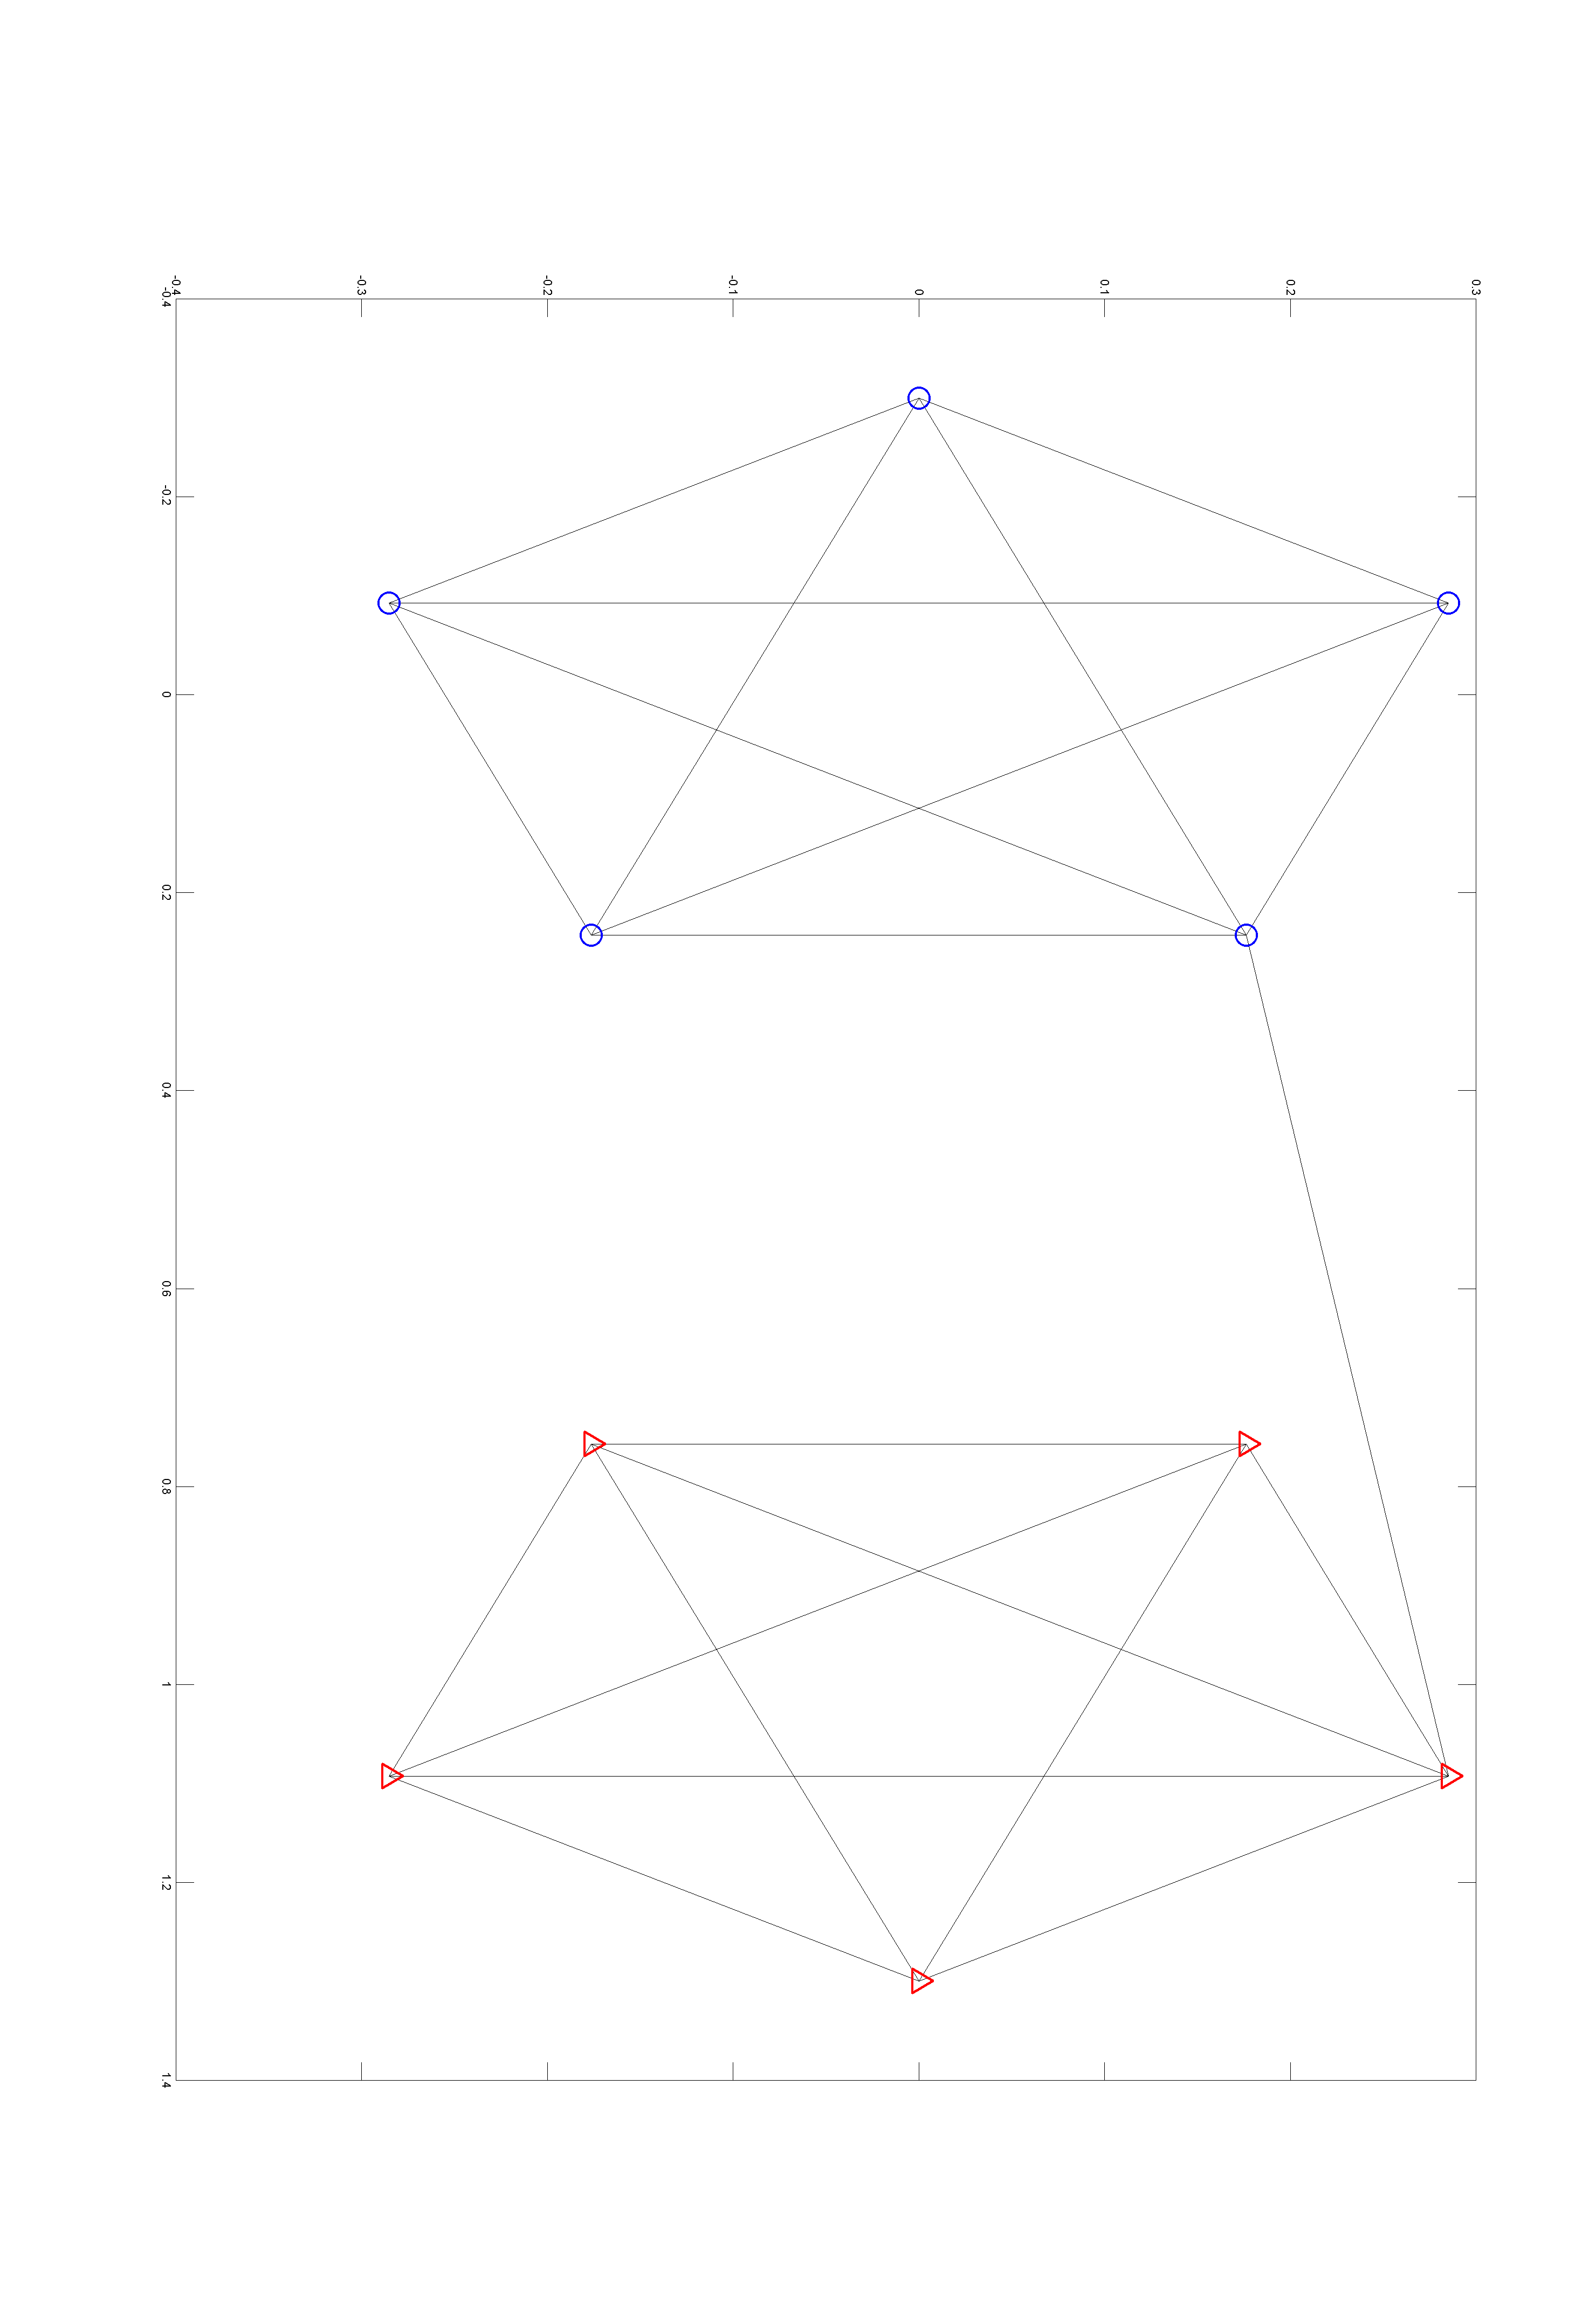
\includegraphics[height=1.5cm,width=2.3cm]{FigNetworks-Clusters.pdf}
        \end{tabular}

        & 2

        & $\left(\begin{array}{cc} 1&\varepsilon\\ \varepsilon&1\\
          \end{array} \right)$ \\
        \hline



        \begin{tabular}{p{2cm}} Hierarchical \end{tabular}

        & \begin{tabular}{c}
          \includegraphics[height=1.5cm,width=2.3cm]{hierarchique.png}
        \end{tabular}

        & 5

        & $\left( \begin{array}{ccccc} 0&1&1&0&0\\ 0&0&0&1&0\\0&0&0&0&1\\0&0&0&0&0\\
        0&0&0&0&0\\
          \end{array} \right)$ \\

    \end{tabular}

    \end{center}

  \end{table}

\end{frame}


\section{Estimation procedure}
\begin{frame}
  \frametitle{Log-Likelihood of the model}
  \textbf{First Idea:} Use maximum likelihood estimators
  \begin{itemize}
  \item \textbf{Complete data likelihood}
    \[
    \mathcal{L}(\Xbf,\Zbf) = \sum_i \sum_q Z_{iq}\ln{\alpha_q} +
    \sum_{i < j} \sum_{q,l} Z_{iq} Z_{jl}
    \ln{b(\pi_{ql},X_{ij})}
    \]
    where $b(\pi_{ql},X_{ij}) = \pi_{ql}^{X_{ij}}
    (1-\pi_{ql})^{(1-X_{ij})}$
    \pause
  \item \textbf{Observed data likelihood}
    \[
    \mathcal{L}(\Xbf) = \ln{\sum_{\Zbf} \exp{\mathcal{L}(\Xbf,\Zbf)}}
    \]
    \pause
  \item observed data likelihood requires a sum over $Q^n$
    terms : \alert{untractable}
  \item EM-like strategies require
    $\Pr(\Zbf|\Xbf)$ : \alert{untractable} (no conditional independence).
  \end{itemize}
\end{frame}


\begin{frame}
  \frametitle{Variational Inference: Pseudo Likelihood}
  \textbf{Main Idea:} Replace \alert{complicated} $\Pr(\Zbf|\Xbf)$ by a \alert{simple} $\RX[\Zbf]$ such that
  $KL(\RX[\Zbf], \Pr(\Zbf|\Xbf))$ is minimal.\bigskip
  \pause
  \begin{itemize}
  \item Optimize in $\RX$ the function $\mathcal{J}(\RX)$ given by :
    \begin{eqnarray*}
      \mathcal{J}(\RX[\Zbf])  & = & \mathcal{L}(\Xbf)  - KL(\RX[\Zbf],
      \Pr(\Zbf|\Xbf)) \\
      & = & \mathcal{H}(\RX[\Zbf]) - \sum_{\Zbf} \RX[\Zbf]  \mathcal{L}(\Xbf,\Zbf)
    \end{eqnarray*}
    \pause
  \item For simple $\RX$, $\mathcal{J}(\RX[\Zbf])$ is tractable, \bigskip
  \item At best, $\RX = \Pr(\Zbf|\Xbf)$ and $\mathcal{J}(\RX[\Zbf])
    = \mathcal{L}(\Xbf)$.
  \end{itemize}
\end{frame}



\begin{frame}
  \frametitle{2 Steps Iterative Algorithm}
  \begin{itemize}
  \item \alert{Step 1} \textbf{Optimize $\mathcal{J}(\RX[\Zbf])$ w.r.t.
    $\RX[\Zbf]$}:
    \begin{itemize}
    \item[\bf{$\rightarrow$}] Restriction to a "comfortable" class of
      functions,
    \item[\bf{$\rightarrow$}] $\RX[\Zbf]=\prod_i h(\Zbf_i;\taubf_i)$, with $h(.;\taubf_i)$ the multinomial
      distribution,
    \item[\bf{$\rightarrow$}] $\tau_{iq}$ is a variational parameter
      to be optimized using a fixed point algorithm:
      \[
      \boxed{
    \tilde{\tau}_{iq} \propto \displaystyle \alpha_q
    \prod_{j \neq i} \prod_{l=1}^Q b(\pi_{ql},X_{ij})^{\tilde{\tau}_{jl}}
      }
      \]
    \end{itemize}
    \bigskip
    \pause
  \item \alert{Step 2} \textbf{Optimize $\mathcal{J}(\RX[\Zbf])$ w.r.t.
    $(\alphabf,\pibf)$}:
    \begin{itemize}
    \item[\bf{$\rightarrow$}] Constraint: $\sum_q \alpha_q =1$
      \[
      \boxed{
    \begin{disarray}{rcl}
      \tilde{\alpha}_q & = & \sum_i \tilde{\tau}_{iq}/n \\
      \tilde{\pi}_{ql} & = &\sum_{ij} \tilde{\tau}_{iq}\tilde{\tau}_{jl}X_{ij}/\sum_{ij} \tilde{\tau}_{iq}\tilde{\tau}_{jl}
    \end{disarray}
      }
      \]
    \end{itemize}
  \end{itemize}
\end{frame}




\begin{frame}
  \frametitle{Model Selection Criterion}
  \begin{itemize}
  \item  BIC-like criterion to select the number of
    classes:\bigskip
  \item The likelihood can be split: $\Lcal(\Xbf, \Zbf |
    Q)=\Lcal(\Xbf | \Zbf,Q)  + \Lcal(\Zbf|Q)$.\bigskip
  \item These terms can be penalized separately:
    \begin{eqnarray*}
      \Lcal(\Xbf | \Zbf,Q) &\rightarrow &
      \text{pen}_{\Xbf|\Zbf}=\frac{Q(Q+1)}{2} \log \frac{n(n-1)}{2} \\
      \Lcal(\Zbf|Q)        &\rightarrow &  \text{pen}_{\Zbf} =
      (Q-1)\log(n)
    \end{eqnarray*}
  \end{itemize}

  \pause
  \begin{center}
    \framebox{$ICL(Q) = \underset{\thetabf}{\max} \Lcal(\Xbf ,
      \tilde{\Zbf} | \thetabf , m_Q) - \frac{1}{2}\left(\frac{Q(Q+1)}{2} \log
      \frac{n(n-1)}{2}- (Q-1) \log(n)\right)$}
  \end{center}
\end{frame}


\section{Examples}
\begin{frame}
\frametitle{Karate Club}
\begin{tabular}{p{6cm}p{5cm}}
  \vspace{1cm}
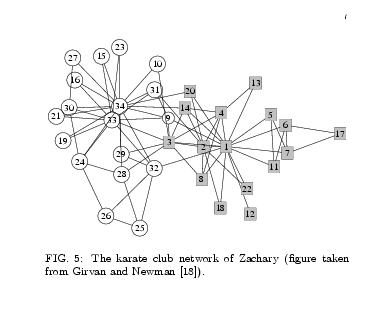
\includegraphics[scale=0.40] {graphe_karate.png} &
\vspace{0cm}\begin{itemize}
    \item nodes are members of the club
    \item edges between 2 members if they have social relation outside the club
    \item known properties: the club has split away in two parts (cercles and squares).
\end{itemize}
{\tiny Data from W. W. Zachary, An information flow model for conflict and fission in small groups, Journal of Anthropological Research 33, 452-473 (1977).}  \\
\end{tabular}

\end{frame}

\begin{frame}
\frametitle{Mixnet results for Karate Club}
\begin{tabular}{p{5cm}p{6cm}}
  \vspace{0cm}
 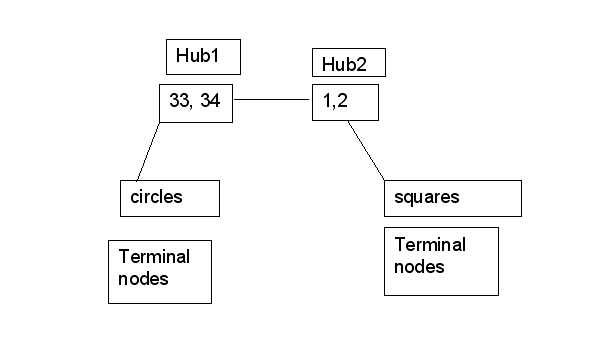
\includegraphics[scale=0.25] {karate-simple.png} &
\vspace{0cm}
 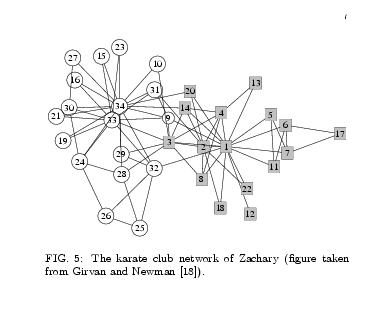
\includegraphics[scale=0.4] {graphe_karate.png}
   \\
  { \small
   \begin{tabular}{|r|rrrr|}
  \hline
 & \multicolumn{4}{c|}{MixNet Classes} \\
 & \alert {1} & 2 & 3 &  4 \\
  \hline
\alert {1} 	&   \alert {100} &  \alert {53} 	&   \alert {16} 	&   \alert {16} 	\\

\setbeamercolor{alerted text}{use=monalerte, fg=monalerte.fg}

\alert{2} 	& \setbeamercolor{alerted text}{use=monalerte, fg=monalerte.fg} \alert{53} 	&  \setbeamercolor{alerted text}{use=monalerte, fg=monalerte.fg} \alert{12} 	&   \setbeamercolor{alerted text}{use=monalerte, fg=monalerte.fg} \alert{0} 	&   \setbeamercolor{alerted text}{use=monalerte, fg=monalerte.fg} \alert{7}  	\\
3 	& 16 	&   0 	&   8 &   73 \\
4 	&   16 	&   7 	&   73 	&   100	\\

\hline
$n*\alpha$ 	& 3 &  13	& 16 	& 2  	\\
   \hline
\end{tabular} }
&  The split is recovered and the role of the leaders is underlined. \\
\end{tabular}

\end{frame}
\setbeamercolor{alerted text}{fg=red} 





\begin{frame}
\frametitle{Transcriptional regulatory network of E. Coli}
\begin{tabular}{p{7cm}p{4cm}}
  \hspace{-1.5cm}
\includegraphics[scale=0.30] {Colinet_base.png} &
\vspace{-6cm}\begin{itemize}
    \item nodes are operons
    \item edges between 2 operons if one regules the other
    \item known properties: sparseness, no feed-back circuits, hierarchical organization.
\end{itemize}
{\tiny Data from Shen-Or et al. Nature genetics, 2002}  \\
\end{tabular}

\end{frame}

\begin{frame}
\frametitle{Mixnet results for RTN of E. Coli}
\begin{tabular}{p{5cm}p{6cm}}
  \vspace{0cm}
 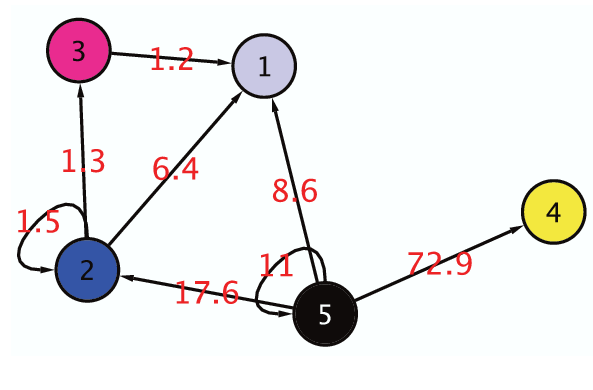
\includegraphics[scale=0.25] {TRN_Q5_summary.png} &
\vspace{0cm}
 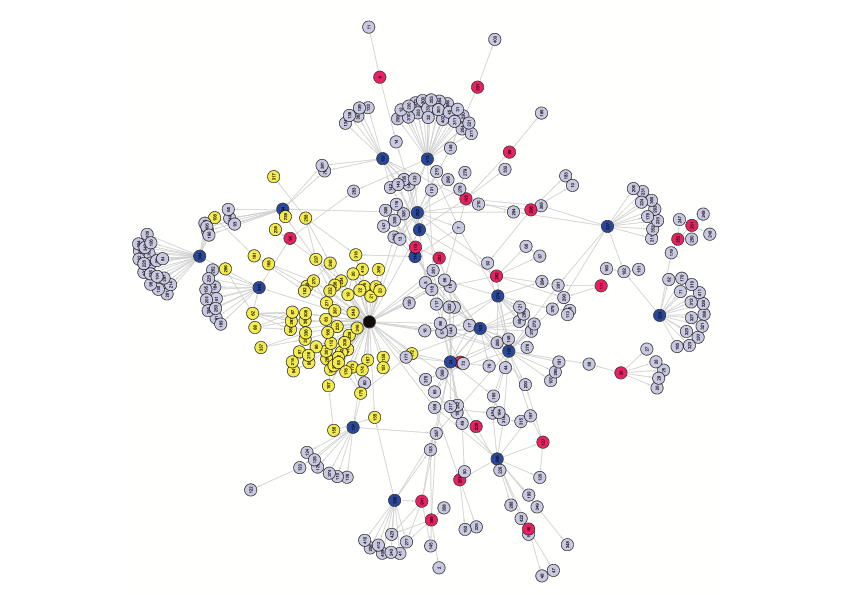
\includegraphics[scale=0.2] {Colinet_Q5.png}
   \\
  { \tiny
   \begin{tabular}{|r|rrrrr|}
  \hline
 & \multicolumn{5}{c|}{MixNet Classes} \\
 & 1 & 2 & 3 & 4 & 5 \\
  \hline
1 	&   . 	&   . 	&   . 	&   . 	&   . 	\\
2 	& 6.40 	& 1.50 	& 1.34 	&   . 	&   . 	\\
3 	& 1.21 	&   . 	&   . 	&   . 	&   . 	\\
4 	&   . 	&   . 	&   . 	&   . 	&   . 	\\
5 	& 8.64 	& 17.65 &   . 	& 72.87 & 11.01 \\
\hline
alpha 	& 65.49 & 5.18 	& 7.92 	& 21.10 & 0.30 	\\
   \hline
\end{tabular} }
&  Meta Hierarchical structure, Meta Single Input Modules and Feed Forward Loops. \\
\end{tabular}

\end{frame}


\begin{frame}
\frametitle{Macaque Cortex Network}
\begin{tabular}{p{7cm}p{4cm}}
  \hspace{-1.5cm}
\includegraphics[scale=0.30] {macaque_base.png} &
\vspace{-6cm}\begin{itemize}
    \item nodes are cortical regions
    \item edges between 2 regions if one is connected to the other
    \item known properties: highly connected network, central and "provincial hubs".
\end{itemize}
{\tiny Data from Sporns et al. PLoS one, 2007}   \\
\end{tabular}

\end{frame}

\begin{frame}
\frametitle{Mixnet results for Cortex network}
\begin{tabular}{p{7cm}p{4cm}}
  \vspace{0cm}
 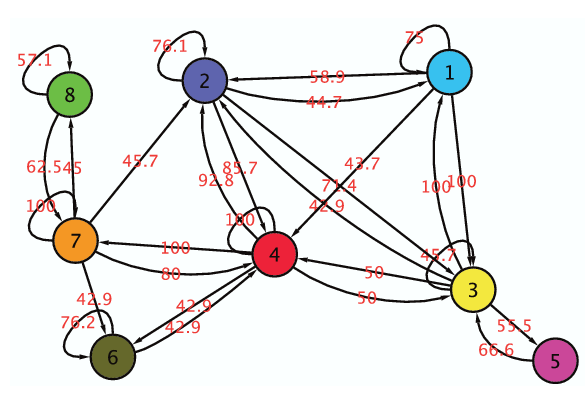
\includegraphics[scale=0.25] {cortex_Q8_summary_lim32.png} &
\hspace{0cm}
 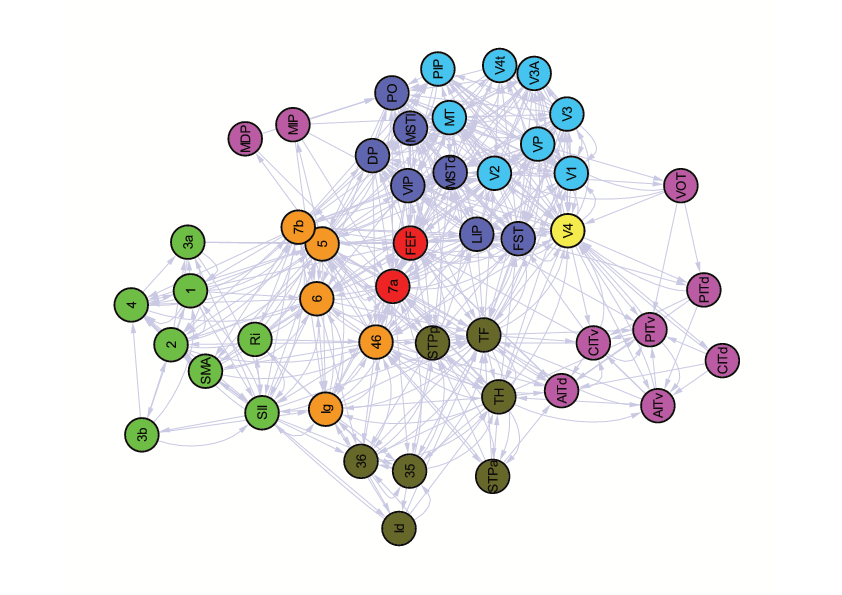
\includegraphics[scale=0.15] {macaque_matrix_Q8.png}
   \\
   \hspace{-1cm} {\tiny
   \begin{tabular}{|r|rrrrrrrr|}
  \hline
 & \multicolumn{8}{c|}{MixNet Classes} \\
 & 1 & 2 & 3 & 4 & 5 & 6 & 7 & 8 \\
  \hline
1 & 75.0 & 58.9 & 100.0 & 43.7 & 2.8 & 3.6 & 10.0 &   . \\
2 & 44.7 & 76.1 & 71.4 & 85.7 & 3.2 & 12.2 & 25.7 &   . \\
3 & 100.0 & 42.9 & 45.7 & 50.0 & 55.5 & 28.6 & 20.0 &   . \\
4 & 6.2 & 92.8 & 50.0 & 100.0 & 11.1 & 42.9 & 100.0 &   . \\
5 & 4.2 & 6.4 & 66.6 & 27.8 & 23.6 & 4.8 & 4.4 &   . \\
6 & 8.9 & 12.2 & 28.6 & 42.9 & 12.7 & 76.2 & 31.4 & 1.8 \\
7 & 15.0 & 45.7 &   . & 80.0 & 6.7 & 42.9 & 100.0 & 45.0 \\
8 &   . &   . &   . & 18.7 &   . & 7.1 & 62.5 & 57.1 \\
\hline
alpha & 17.0 & 14.9 & 2.1 & 4.3 & 19.2 & 14.9 & 10.6 & 17.0 \\
   \hline
\end{tabular} }
&  Central and provincial  hubs well identified. \\
\end{tabular}

\end{frame}


\begin{frame}
\frametitle{Food-web network}
\begin{tabular}{p{5cm}p{6cm}}
  \hspace{-1cm} \vspace{5cm}
\includegraphics[scale=0.20, angle=0] {grass_web_base.png} &
\vspace{-3cm}\begin{itemize}
    \item the food web shows 5 levels of organization: plants (circle), herbivores (box),
parasitoids (parallelogram), hyperparasitoids (triangle) and hyper-hyperparasitoids (diamond).
    \item a trophic link is considered
between two insects when one insect is observed within one host
    \item known properties: hierarchic organization.
\end{itemize}
{\tiny Data from Dawah et al. Journal of animal ecology, 1995, and Martinez et al. Ecology, 1999}  \\
\end{tabular}

\end{frame}

\begin{frame}
\frametitle{Mixnet results for Food-Web network}
\begin{tabular}{p{6cm}p{5cm}}
  \hspace{-1cm}
 \includegraphics[height=4cm,width=7cm] {grass_web_Q7_summary.png} &
\vspace{-4cm}
 \includegraphics[scale=0.2, angle=0] {grass_web_Q7.png}
   \\
  \hspace{-1cm} { \tiny
   \begin{tabular}{|r|rrrrrrr|}
  \hline
 & \multicolumn{7}{c|}{MixNet Classes} \\
 & 1 & 2 & 3 & 4 & 5 & 6 & 7 \\
  \hline
1 &   . &   . & 16.3 &   . &   . &   . &   . \\
  2 & 10.6 &   . &   . &   . &   . &   . &   . \\
  3 &   . &   . &   . &   . &   . &   . &   . \\
  4 &   . &   . & 2.3 & 6.3 &   . &   . &   . \\
  5 &   . &   . & 2.6 &   . & 30.0 &   . &   . \\
  6 & 90.2 & 22.6 &   . &   . &   . &   . &   . \\
  7 & 19.2 &   . &   . & 53.5 &   . &   . &   . \\
\hline
  alpha & 14.0 & 44.4 & 8.6 & 22.3 & 8.0 & 1.3 & 1.3 \\
   \hline
\end{tabular}} &  The 5 levels are well identified plus a specific community. Local hierarchies are detected. \\
\end{tabular}

\end{frame}

\begin{frame}
\frametitle{Conclusions}
\begin{itemize}
  \item Mixnet is a flexible model which allows to replace a complicated network by a simple meta-network.
  \item Freely available package, URL: http://pbil.univ-lyon1.fr/software/MixNet.
  \item Extension to Poisson and Gaussian $X$ is already made.
  \item properties of variational estimates is in progress
\end{itemize}

More details :  J.J. Daudin, F. Picard, and S. Robin. A mixture model for random graphs. Stat and
Computing, 18, 2008.
\end{frame}

\begin{frame}
\frametitle{Common work with}

\begin{tabular}{|c|c|c|c|}
  \hline
  % after \\: \hline or \cline{col1-col2} \cline{col3-col4} ...
  Franck Picard & \includegraphics[scale=0.2, angle=0] {PicardF.jpg} & {\tiny  UMR CNRS 5558,UCB Lyon 1 } & {\tiny Method+Biological examples+Mixnet package} \\
  \hline
  Vincent Miele & \includegraphics[scale=0.2, angle=0] {MieleV.png} & {\tiny  UMR CNRS 5558,UCB Lyon 1 } &{\tiny Mixnet package} \\
  \hline
   St�phane Robin & \includegraphics[scale=0.6, angle=0] {RobinS.jpg} & {\tiny UMR 518 AgroParisTech/INRA}& {\tiny Method} \\
   \hline
   Mahendra Mariadassou &  & {\tiny UMR 518 AgroParisTech/INRA}& {\tiny Method} \\
   \hline
   Ludovic Cottret &  \includegraphics[scale=0.2, angle=0] {CottretL.jpg} & {\tiny  UMR CNRS 5558,UCB Lyon 1 } & {\tiny Mixnet package}\\
  \hline
\end{tabular}

\end{frame}





%******************************************************************************




\begin{frame}
\frametitle{Why do people represent data by a network (3) ?}
\begin{tabular}{p{6cm}p{5cm}}
  \hspace{-1cm}
\includegraphics[scale=0.20] {Framingham_heart_study.png} &
\vspace{-5cm}\begin{itemize}
    \item nodes may be of different sizes, adding more information
    \item edges may be colored, adding more information
    \item a movie may report the evolution of the network in time.
\end{itemize}     \\
\end{tabular}
{\tiny  2200 persons (nodes) from the Framingham Heart study.
Circles with red borders = women, circles with blue borders = men.
The size of each circle is proportional to BMI. The color of the
circles indicates the person's obesity status: yellow = obese
person  and green = nonobese person. The colors of the ties
between the nodes indicate the relationship between them: purple
denotes a friendship or marital tie and orange denotes a familial
tie. N.A. Christakis et al. N Engl J Med, 2007, July}
\end{frame}


\begin{frame}
\frametitle{Research Fronts rankings in Mathematics, {\small sorted by
Citations}} {\small ISI WEB of Knowledge Essential Science Indicators \\
\begin{tabular}{|p{1cm}|p{4cm}|p{1cm}|p{1cm}|p{1cm}|p{1cm}|}
  % after \\: \hline or \cline{col1-col2} \cline{col3-col4} ...
  \hline
{\small Rank}   & Research Front &  {\tiny Core Papers} & {\tiny Citations} & {\tiny Citations / paper }& {\tiny Mean year} \\
\hline
  1 & {\small \alert {Complex networks}, Statistical mechanics, Structure, Function, Evolution}  & 3 & 3415 & 1138 & 2002.3 \\
   \hline
  2 & {\small Current-driven magnetic domain wall motion}  & 27 & 1385 & 51.3 & 2004.6
  \\ \hline
  3 & {\small False discovery rate procedure } & 9 & 936 & 104 & 2003.3
  \\ \hline
  4 & {\small Evolutionary game dynamics, \alert {Social networks}}  & 12 & 382 & 31.83 & 2004.8
  \\ \hline
  5 & {\small Porous plate using homotopy analysis method}  & 12 & 359 & 29.92 & 2003.7 \\
  \hline
\end{tabular}
}
\end{frame}


\begin{frame}

\frametitle{System Biology}

{\bf Biological systems} show emergent properties that are not
readily explainable by the study of their constituent parts...

 {\bf New mathematical formalisms}, based on
graph theory, are emerging in order to represent and study the
underlying interaction networks present in the cell.

The understanding of the {\bf evolution and organization of these
networks} is changing the way scientists look at biology.

 More specifically:
 \begin{itemize}

 \item gene regulation
 \item metabolic pathways analysis
 \item protein-protein interactions
 \end{itemize}
\end{frame}

\begin{frame}
\frametitle{Representations of a correlation matrix by a graph}
{\small
\begin{tabular}{p{3.5cm} p{3.5cm} p{3.5cm}}
  % after \\: \hline or \cline{col1-col2} \cline{col3-col4} ...
  \vspace{-2.5cm}
 \begin{equation*}
     \left(%
\begin{array}{cccc}
  1 & 0.8 & 0.5 & 0.2 \\
   & 1 & 0.1 & 0.1 \\
   &  & 1 & 0.1 \\
   &  &  & 1 \\
\end{array}%
\right)
\end{equation*} & \includegraphics[height=2.5cm ]
{Graphe-Correlation_value.png} &
 \includegraphics[height=2.5cm ] {Graphe-Correlation_binaire.png} \\

  Correlation matrix& Valued graph & Binary graph using 0.15 threshold \\
  Not readable if more than 10 items & Not readable if more than 10 items & Clusters and hubs appears,
   but the result depends on the threshold used and the representation software. \\
\end{tabular}
Other graphical representations are possible: colored intensity
matrix, PCA... }
\end{frame}


\begin{frame}
\frametitle{The focus is on topological questions}

\begin{tabular}{p{7.5cm}p{5cm}}

\vspace{0cm} \hspace{0cm}{\small  Are there clusters of similar nodes?
     \begin{itemize}
        \item
     existence of
    functional modules in biological networks, i.e.  sub-networks
    which can produce outputs independently.
        \item
        Each cluster may be studied independently and thus
        we are allowed to work on lower sized networks.
        \item If a node A, with unknown properties, is in the same cluster that a
        well known node B, then we are tempted to attribute B's properties to
        A.
        \item How many hubs ? they are the most important nodes
    in the network.
     \item Resilience of the network's connectivity to edge suppression.
    \end{itemize}}
    &
     \vspace{0cm} \hspace{-2.5cm}
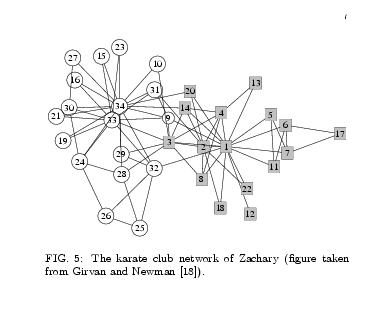
\includegraphics[scale=0.3, angle=-90]{graphe_karate.pdf} \\
\end{tabular}

\end{frame}


\begin{frame}
\frametitle{Clustering methods}
\begin{description}
    \item[Hierarchical clustering] a well-known set of algorithms
    for a similarity matrix, many criteria proposed
    \item[Spectral clustering]: k-means on the space associated to the $q$-lowest eigenvalues of the Laplacian
    of the network, $D-X$, with $D=diag(sum(X))$ {\tiny tutorial from U. Von Luxburg, Stat Comput,
    2007}.
    \item[Markov Clustering Algorithm] MCL simulates a flow on the
    graph by calculating successive powers of $X$. At each
    iteration an inflation step is applied to enhance the contrast
    between regions of strong or weak flow in the graph. The
    process converges towards a partition of the graph, with a set
    of high flow regions separated by boundaries with no flow,
    {\tiny package from Von Dongen}
    \item[Edge-betweenness clustering] Divisive method using the
edge betweenness EB, (for an edge) : the number of shortest paths
that pass through the edge. The edge with the highest EB is
removed, {\tiny  Girvan \& Newman}
\end{description}
\end{frame}

\begin{frame}
\frametitle{Clustering of nodes}

\includegraphics[scale=0.5, angle=0]{communities.png} \\
Santa Fe Institute collaboration network: the nodes of the network
represent scientists from the Santa Fe Institute and an edge is
drawn between two nodes if the corresponding scientists have
coauthored at least one publication during the calendar year 1999
or 2000.

\end{frame}

\begin{frame}
\frametitle{Statistical models for networks}
\end{frame}

\begin{frame}
\frametitle{Statistical models for networks} More probabilistic
models for networks are necessary to:\begin{enumerate}
    \item summarize the information contained in one network and
    compare networks
    \item have a reference model to say if a particular motif is
    exceptional
    \item predict the label of a node
    \item predict the value of an edge
    \item create artificial networks by simulation
\end{enumerate}
\end{frame}

\end{document}
